\documentclass[border=4pt]{standalone}
\usepackage{tikz}
\usetikzlibrary{arrows.meta,positioning,shapes.geometric}
\begin{document}
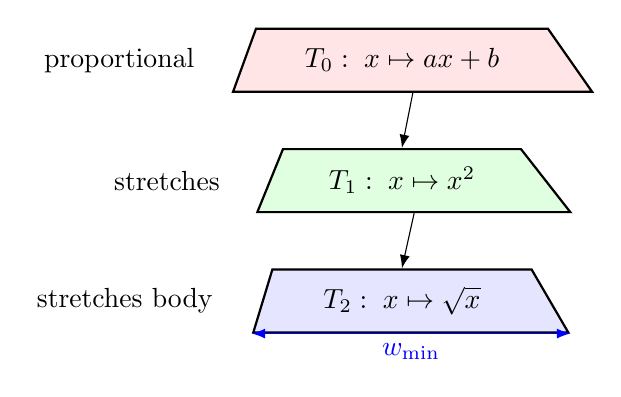
\begin{tikzpicture}[
  node distance=7mm,
  >=Latex,
  sample/.style={
    trapezium,
    draw,
    thick,
    trapezium left angle=70,
    trapezium right angle=55,
    minimum width=40mm,
    minimum height=8mm,
    inner sep=1.5mm
  }
]
  \node[sample,fill=red!10] (similar) {$T_0:\;x\mapsto ax+b$};
  \node[sample,trapezium stretches,fill=green!12,below=of similar]
    (independent) {$T_1:\;x\mapsto x^2$};
  \node[sample,trapezium stretches body,fill=blue!10,below=of independent]
    (body) {$T_2:\;x\mapsto \sqrt{x}$};

  \draw[-Latex] (similar.bottom side) -- (independent.top side);
  \draw[-Latex] (independent.bottom side) -- (body.top side);
  \draw[<->,blue] (body.bottom left corner) -- (body.bottom right corner)
    node[midway,below] {$w_{\min}$};
  \node[left=5mm of similar] {proportional};
  \node[left=5mm of independent] {stretches};
  \node[left=5mm of body] {stretches body};
\end{tikzpicture}
\end{document}
